\documentclass[12pt,dvips]{article}
\usepackage{epsfig}
\usepackage{html}
\newcommand{\oofem}{\htmladdnormallink{OOFEM}{http://www.oofem.org}\ }
\newcommand{\bp}{\htmladdnormallink{Bo\v{r}ek Patz\'{a}k}{http://mech.fsv.cvut.cz/~bp/bp.html}}
\newcommand{\mbf}[1]{\mbox{\boldmath$#1$}}
\newcommand{\descitem}[1]{{\noindent \bf #1}:}
\newcommand{\elemkeyword}[1]{\descitem{Keyword}~{\em #1}}
\newcommand{\elemparam}[2]{{{#1\tiny (#2)}~~\#}}
\newcommand{\optelemparam}[2]{{[~\elemparam{#1}{#2}]}}
\newcommand{\param}[1]{{\it #1}}



\begin{document}
%begin{latexonly}
\title{\oofem Element Library Manual}
\author{\bp \\ \\
Czech Technical University\\
Faculty of Civil Engineering\\
Department of Structural Mechanics\\
Th\'akurova 7, 166 29 Prague, Czech Republic
}
\maketitle
%end{latexonly}
\begin{htmlonly}
\begin{center}
{\Large \oofem Element Library Manual}
{\bp \\ \\
Czech Technical University\\
Faculty of Civil Engineering\\
Department of Structural Mechanics\\
Th\'akurova 7, 166 29 Prague, Czech Republic
}
\end{htmlonly}
\newpage
\tableofcontents
\listoffigures

\section{Introduction}
In this manual the detailed description of available elements 
is given. The actual availibility of particular elements depends on
OOFEM configuration. Elements are specified using element records,
which are part of oofem input file. The general format of element
record is described in OOFEM input manual. 

Every element is desribed in separate section. The section includes the ``element keyword'' which
determines the element type in element record, approximation and
interpolation characteristics, required cross section properties
(which are summarized in ``CS properties'' part), and summary of
element fatures. The ``Load'' section contains usefull
information about the types of loadings supported by particular elements.



\section{Elements for Structural Analysis (SM Module)}
\subsection{Truss Elements}

\subsubsection{Truss 1d element}
\label{Truss1d}

Represents linear isoparametric truss element in 1d. The elements are
assumed to be located along x-axis. Reqiures cross section area to be
specified.

\elemkeyword{truss1d}\\
\descitem{Parameters} none.\\
\descitem{Unknowns}
Single dof (u-displacement) is required in each node .

\descitem{Approximation} Linear approximation of displacement (u) and geometry.

\descitem{Integration} Exact.

\descitem{Features} Full dynamic analysis support, Full nonlocal
constitutive support, Adaptivity support

\descitem{CS properties} Area is required.

\descitem{Loads} Body loads are supported. Boundary loads are
not supported in current implementation.

\descitem{Status} Reliable

\subsubsection{Truss 2d element}
\label{Truss2d}

Two node linear isoparametric truss element for 2d analysis. The
element geometry can be specified in (x,z), (x,y), or (y,z) plane. 
\begin{figure}[tb]
\centerline{\epsfbox{truss2d.eps}}
\caption{Truss2d element in (x,z) plane.}
\end{figure}

\elemkeyword{truss2d}\\
\descitem{Parameters} \optelemparam{cs}{in}\\

\descitem{Unknowns}
Two dofs representing displacements in definition plane are required
in each node. The element can be used in different planes, default
definition plane is (x,z). The parameter \param{cs} can be used to
change default definition plane. The supported values of parametrer
\param{cs} are following: 0 for (x,z) plane (default), 1 for (x,y)
plane, and 3 for (y,z) plane.

\descitem{Approximation} Linear approximation of displacements and geometry.

\descitem{Integration} Exact.

\descitem{Features} Full dynamic analysis support. Full nonlocal
constitutive support.

\descitem{CS properties} cross section area should be
provided.

\descitem{Loads} Edge loads are supported, Edge number should be equal
to 1.

\descitem{Status} Reliable

\subsection{Beam Elements}
\subsubsection{Beam2d element}
Beam element for 2d analysis, based on Timoshenko hypothesis. Structure should be defined in x,z
plane. The internal condensation
of arbitrary DOF is supported and is performed in local coordinate
system. On output, the local end displacement and local end forces are
printed. 

\begin{figure}[tb]
\begin{center}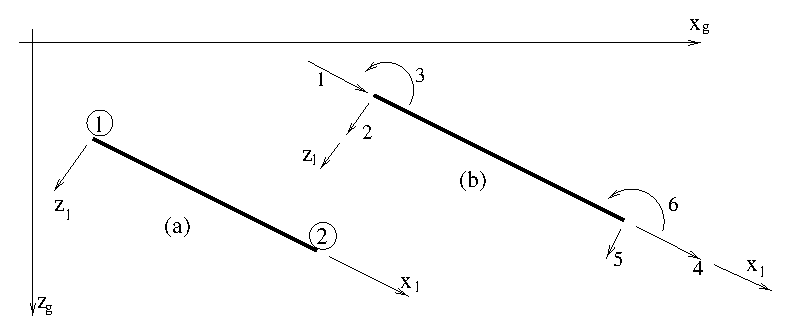
\epsfig{file=beam2d.eps,width=120mm}\end{center}
\caption{Beam2d element. Definition of local c.s.(a)  and definition of
local end forces and local element dofs (b).}
\label{beam2dfig}
\end{figure}

\elemkeyword{beam2d}\\
\descitem{Parameters} \optelemparam{dofstocondense}{ia}. The
\param{dofstocondense} parameter allows to specify local element dofs that
will be condensed. The numbering of local element dofs is shown in
fig.~\ref{beam2dfig}. The size of this array should be equal to
number of local element dofs (6) and nonzero value indicates the
corresponding dof will be condensed.\\
\descitem{Unknowns}
Three dofs (u-displacement, w-displacement, y-rotation) are required
in each node.\\
\descitem{Approximation} Cubic  approximations of lateral displacement and
rotation are used. For longitudinal displacement the linear one is
assumed.\\
\descitem{Integration} Exact.\\
\descitem{Features} Full dynamic analysis support. Linear stability
analysis support.\\
\descitem{CS properties} Area,
inertia moment along y-axis and area shear correction factor should be specified.\\ 
\descitem{Loads}  Constant and linear edge loads are supported, shear
influence is taken into account. 
Edge number should be equal to 1. Temperature load is
supported, the first coefficient of temperature load represent
mid-plane temperature change, the second one represent difference
between temperature change of local z+ and local z- surfaces of beam (in local coordinate
system). Temperature load require that the ``thick'' property of cross
section model is defined.

\descitem{Status} Reliable.

\subsubsection{Beam3d element}
Beam element for 3d {\bf linear} analysis, based on Timoshenko hypothesis. The internal condensation
of arbitrary DOF is supported and is performed in local coordinate
system. On output, the local end-displacement and local end-forces are
printed. Requires the local coordinate system to be chosen according
to main central axes of inertia. Local element 
coordinate system is determined by the following rules:
\begin{enumerate}
\item let first element node has following coordinates $(x_i, y_i, z_i)$
and the second one $(x_j, y_j, z_j)$,
\item direction vector of local x-axis is then $\mbf{a_1} = (x_j-x_i, y_j-y_i, z_j-z_i)$,
\item local y-axis direction vector lies in plane defined by local
x-axis direction vector ($\mbf{a_1}$) and given
point (k-node with coordinates $(x_k, y_k, z_k)$) - so called reference node,
\item local z-axis is then determined as vector product of local
x-axis direction vector ($\mbf{a_1}$) by vector $(x_k-x_i, y_k-y_i, z_k-z_i)$,
\item local y-axis is then determined as vector product of local
z-axis direction vector by local x-axis direction vector. 
\end{enumerate}
\begin{figure}[tb]
\begin{center}\epsfbox{beam3d.eps}\end{center}
\caption{Beam3d element. Definition of local c.s., local end forces
and local element dofs numbering.}
\label{beam3dfig}
\end{figure}

\elemkeyword{beam3d}\\
\descitem{Parameters} \elemparam{refnode}{in}
\optelemparam{dofstocondense}{ia}. The \param{refnode} parameter
determines the reference node. It determines the local coordinate
system of beam element. The \param{dofstocondense} parameter allows to
specify local element dofs that will be condensed. The numbering of
local element dofs is shown in fig.~\ref{beam3dfig}. The size of this
array should be equal to number of local element dofs (12) and nonzero
value indicates the corresponding dof will be condensed.\\
\descitem{Unknowns}
Six dofs (u,v,w-displacements and x,y,z-rotations) are required in each node.\\
\descitem{Approximation} Cubic  approximations of lateral displacement and
rotation (along local y,z axes) are used. For longitudinal displacement
and the rotation along local x-axis (torsion) the linear
approximations are assumed.\\
\descitem{Integration} Exact.\\
\descitem{Features} Full dynamic analysis support. Linear stability
analysis support.\\
\descitem{CS properties} Area, inertia moment along y and z axis, torsion inertia moment and 
cross section area shear correction factor are required. These
cross section properties are assumed to be defined in local coordinate
system of element.\\
\descitem{Loads}  Constant and linear edge loads are supported.
Edge number should be equal to 1. Temperature load is
supported, the first coefficient of temperature load represent
mid-plane temperature change, the second one represent difference
between temperature change of local z+ surface and local
z- surface surface of beam and the third one represent difference
between temperature change of local y+ surface and  local
y- surface of beam. Requires the ``thick'' (measured in direction of
local z axis) and ``width'' (measured in direction of local y axis) cross section
model properties to be defined.\\
\descitem{Status} Stable, various loadings require further testing.

\subsection{Plane Stress Elements}
\subsubsection{PlaneStress2d}
Represents isoparametric four-node quadrilateral plane-stress
finite element. Each node has 2 degrees of freedom.
Structure should be defined in x,y plane. 
The nodes should be numbered anti-clockwise (positive rotation around
z-axis). 

\begin{figure}[tb]
\begin{center}\epsfbox{planestress2d.eps}\end{center}
\caption{PlaneStress2d element. Node numbering, Side numbering and
definition of local edge c.s.(a).}
\label{Planestress2dfig}
\end{figure}

\elemkeyword{planestress2d}\\
\descitem{Parameters} \optelemparam{NIP}{in}\\
\descitem{Unknowns}
Two dofs (u-displacement, v-displacement) are required in each node.

\descitem{Approximation} Linear approximation of displacement and
geometry.

\descitem{Integration}
Integration of membrane strain terms using gauss integration formula
in 4 (the default), 9, or 16 integration points. The default number of
integration point used can be overloaded using \param{NIP} parameter.
Reduced integration for shear terms is employed. Shear terms are
always integrated using 1 point integration rule.

\descitem{Features} Nonlocal constitutive support.

\descitem{CS properties} Thickness. 

\descitem{Loads} Body loads are supported. Boundary loads are
supported and computed using numerical integration. The side numbering is
following. Each i-th element side begins in i-th element node and
ends on next element node (i+1-th node or 1-st node, in the case of 
side number 4). The local positive edge x-axis coincides with side
direction, the positive local edge y-axis is rotated 90 degrees
anti-clockwise (see fig. (\ref{Planestress2dfig})).

\descitem{Status} Reliable.

\subsubsection{QPlaneStress2d}

Implementation of quadratic isoparametric eight-node quadrilateral
plane-stress  finite element. Each node has 2 degrees of freedom.
The node numbering is anti-clockwise and is explained in fig. (\ref
{qplanstrssfig}).

\begin{figure}[htb]
\begin{center}\epsfbox{qplanstrss.eps}\end{center}
\caption{QPlaneStress element - node numbering.}
\label{qplanstrssfig}
\end{figure}

\elemkeyword{qplanestress2d}\\
\descitem{Parameters} \optelemparam{NIP}{in}\\
\descitem{Unknowns}
Two dofs (u-displacement, v-displacement) are required in each node.

\descitem{Approximation} Quadratic approximation of displacement and
geometry.

\descitem{Integration}
Full integration using gauss integration formula
in 4 (the default), 9, or 16 integration points. The default number of
integration point used can be overloaded using \param{NIP} parameter.

\descitem{Features} Adaptivity support.

\descitem{CS properties} Thickness. 

\descitem{Loads} Body loads are supported. Boundary loads are
not supported in current implementation.

\descitem{Status} Stable.

\subsubsection{TrPlaneStress2d}
Implements an triangular three-node  constant strain plane-stress  
finite element. Each node has 2 degrees of freedom.
The node numbering is anti-clockwise

\begin{figure}[htb]
\begin{center}\epsfbox{trplanstrss.eps}\end{center}
\caption{TrPlaneStress element - node and side numbering.}
\label{TrPlanestressfig}
\end{figure}

\elemkeyword{trplanestress2d}\\
\descitem{Parameters} none.\\
\descitem{Unknowns}
Two dofs (u-displacement, v-displacement) are required in each node.

\descitem{Approximation} Linear approximation of displacement and
geometry.

\descitem{Integration}
Integration of membrane strain terms using one point gauss integration formula.

\descitem{Features} Nonlocal constitutive support, Edge load
support, Geometrical nonlinearity support, Adaptivity support

\descitem{CS properties} Thickness. 

\descitem{Loads} Body loads are supported. Boundary loads are
supported and are computed  using numerical integration. The side numbering is
following. Each i-th element side begins in i-th element node and
ends on next element node (i+1-th node or 1-st node, in the case of 
side number 3). The local positive edge x-axis coincides with side
direction, the positive local edge y-axis is rotated 90 degrees
anti-clockwise (see fig. (\ref{TrPlanestressfig})).

\descitem{Status} Reliable.

\subsubsection{QTrPlStr}
Implementation of quadratic six-node plane-stress finite
element. Each node has 2 degrees of freedom. Node numbering is
anti-clockwise and is shown in fig. (\ref{qtrplanstressfig}).

\begin{figure}[htb]
\begin{center}\epsfbox{qtrplanstrss.eps}\end{center}
\caption{TrPlaneStress element - node and side numbering.}
\label{qtrplanstressfig}
\end{figure}

\elemkeyword{qtrplstr}\\
\descitem{Parameters} \optelemparam{NIP}{in}.\\
\descitem{Unknowns}
Two dofs (u-displacement, v-displacement) are required in each node.

\descitem{Approximation} Quadratic approximation of displacement and
geometry.

\descitem{Integration}
Full integration using gauss integration formula in 4 points (the
default) or in 7 points (using \param{NIP} parameter).

\descitem{Features} Adaptivity support (error indicator).

\descitem{CS properties} Thickness. 

\descitem{Loads} 

\descitem{Status} 

\subsubsection{TrPlaneStrRot}
Implementation of triangular three-node  plane-stress 
finite element with independent rotation field.
Each node has 3 degrees of freedom.

\elemkeyword{trplanestrrot}\\
\descitem{Parameters} \optelemparam{NIP}{in} \optelemparam{NIPRot}{in}.\\
\descitem{Unknowns}
Three dofs (u-displacement, v-displacement, z-rotation) are required in each node.

%\descitem{Approximation}

\descitem{Integration}
Integration of membrane strain terms using gauss integration formula
in 4 points (default) or using 1or 7 points (using \param{NIP} parameter).
Integration of strains associated with rotational field 
integration using 1 point is default (4 and 7 points rules can be
specified using \param{NIPRot} parameter).

\descitem{CS properties} Thickness. 

\descitem{Features} 

\descitem{Status} 

\subsection{Plane Strain Elements}

\subsubsection{Quad1PlaneStrain}
Represents isoparametric four-node quadrilateral plane-strain
finite element. Each node has 2 degrees of freedom.
Structure should be defined in x,y plane. 
The nodes should be numbered anti-clockwise (positive rotation around
z-axis). 

\begin{figure}[tb]
\begin{center}\epsfbox{planestress2d.eps}\end{center}
\caption{Quad1PlaneStrain element. Node numbering, Side numbering and
definition of local edge c.s.(a).}
\label{Quad1PlaneStrainfig}
\end{figure}

\elemkeyword{quad1planestrain}\\
\descitem{Parameters} \optelemparam{NIP}{in}\\
\descitem{Unknowns}
Two dofs (u-displacement, v-displacement) are required in each node.

\descitem{Approximation} Linear approximation of displacement and
geometry.

\descitem{Integration}
Integration of membrane strain terms using gauss integration formula
in 4 (the default), 9, or 16 integration points. The default number of
integration point used can be overloaded using \param{NIP} parameter.
Reduced integration for shear terms is employed. Shear terms are
always integrated using 1 point integration rule.

\descitem{Features} Nonlocal constitutive support, Adaptivity support.

\descitem{CS properties} Thickness. 

\descitem{Loads} Body loads are supported. Boundary loads are
supported and computed using numerical integration. The side numbering is
following. Each i-th element side begins in i-th element node and
ends on next element node (i+1-th node or 1-st node, in the case of 
side number 4). The local positive edge x-axis coincides with side
direction, the positive local edge y-axis is rotated 90 degrees
anti-clockwise (see fig. (\ref{Quad1PlaneStrainfig})).

\descitem{Status} Reliable.


\subsubsection{TrplaneStrain}
Implements an triangular three-node  constant strain plane-strain  
finite element. Each node has 2 degrees of freedom.
The node numbering is anti-clockwise

\begin{figure}[htb]
\begin{center}\epsfbox{trplanstrain.eps}\end{center}
\caption{TrplaneStrain element - node and side numbering.}
\label{TrplaneStrain}
\end{figure}

\elemkeyword{trplanestrain}\\
\descitem{Parameters} none.\\
\descitem{Unknowns}
Two dofs (u-displacement, v-displacement) are required in each node.

\descitem{Approximation} Linear approximation of displacement and
geometry.

\descitem{Integration}
Integration of membrane strain terms using one point gauss integration formula.

\descitem{Features} Nonlocal constitutive support. Edge load
support, Adaptivity support.

\descitem{CS properties} Thickness. 

\descitem{Loads} Body loads are supported. Boundary loads are
supported and are computed  using numerical integration. The side numbering is
following. Each i-th element side begins in i-th element node and
ends on next element node (i+1-th node or 1-st node, in the case of 
side number 3). The local positive edge x-axis coincides with side
direction, the positive local edge y-axis is rotated 90 degrees
anti-clockwise (see fig. (\ref{TrplaneStrain})).

\descitem{Status} Reliable.



\subsection{Plate\&Shell Elements}
\subsubsection {CCT Element}
Implementation of constant curvature triangular element for plate
analysis. Formulation based on Mindlin hypothesis. The structure should be defined in x,y plane. 
The nodes should be numbered anti-clockwise (positive rotation around
z-axis). 


\elemkeyword{cctplate}\\
\descitem{Parameters} none.\\
\descitem{Unknowns}
Three dofs (w-displacement, u and v - rotation) are required in each node.

%\descitem{Approximation} 

\descitem{Integration}
Integration of all terms using one point formula.

\descitem{Features} Layered cross section support.

\descitem{Loads} Body loads are supported. Boundary loads are
not supported now.

\descitem{Status} Reliable.

\subsubsection {RerShell Element}
Combination of CCT plate element (Mindlin hypothesis) with triangular plane stress element
for membrane behavior. The element curvature can be specified. 
Although element requires generally six dofs per node, no stiffness to
local rotation along z-axis (rotation around element normal) is supplied.

\elemkeyword{rershell}\\
\descitem{Parameters} none.\\
\descitem{Integration}
Integration of all terms using one point formula.\\
\descitem{Features} Layered cross section support.\\
\descitem{Loads} Body loads are supported. Boundary loads are
not supported now.\\
\descitem{Status} Reliable.

\subsection{Axisymmetric Elements}
\subsubsection{Axisymm3d element}
Implementation of triangular three-node finite element 
for axisymmetric continuum. Each node has 2 degrees of freedom.
\elemkeyword{axisymm3d}\\
\descitem{Parameters} \optelemparam{NIP}{in} \optelemparam{NIPfish}{in}.\\
\descitem{Unknowns}
Two dofs (u-displacement, v-displacement) are required in each node.
\descitem{Approximation} Linear approximation of displacement and
geometry.
\descitem{Integration}
The integration of $\varepsilon_x$ and $\varepsilon_y$ strains can be altered using
\param{NIP} parameter (possible completions are 1 (default), 4 and 7
point integration rule). The remaining strain components ($\varepsilon_\phi$ and
$\gamma_rz$) can be integrated using 1 (default), 4 and 7 integration
point formulae (\param{NIPfish} parameter).\\
\descitem{Features} None.\\
\descitem{Loads} No boundary and body loads are supported.\\
\descitem{Status} 

\subsubsection{Q4axisymm element}
Implementation of quadratic isoparametric eight-node quadrilateral -
finite element for axisimmetric 3d continuum. 
Each node has 2 degrees of freedom.

\elemkeyword{q4axisymm}\\
\descitem{Parameters} \optelemparam{NIP}{in} \optelemparam{NIPfish}{in}.\\
\descitem{Unknowns}
Two dofs (u-displacement, v-displacement) are required in each node.
\descitem{Approximation} Quadratic approximation of displacements and
geometry.
\descitem{Integration}
The integration of $\varepsilon_x$ and $\varepsilon_y$ strains can be altered using
\param{NIP} parameter (possible completions are 1 (default), 4, 9 and 16
point integration rule). The remaining strain components ($\varepsilon_\phi$ and
$\gamma_rz$) can be integrated using 1 (default), 4, 9 and 16 integration
point formulae (\param{NIPfish} parameter).\\
\descitem{Features} None.\\
\descitem{Loads} No boundary and body loads are supported.\\
\descitem{Status} 

\subsubsection{L4axisymm element}
Implementation of isoparametric four-node quadrilateral axisymmetric
finite element. Each node has 2 degrees of freedom.

\elemkeyword{l4axisymm}\\
\descitem{Parameters} \optelemparam{NIP}{in}. \\
\descitem{Unknowns}
Two dofs (u-displacement, v-displacement) are required in each node.
\descitem{Approximation} Linear approximation of displacements and
geometry.
\descitem{Integration}
The integration of $\varepsilon_x$ and $\varepsilon_y$ strains can be altered using
\param{NIP} parameter (possible completions are 1 (default), 4, 9 and 16
point integration rule). The remaining strain components ($\varepsilon_\phi$ and
$\gamma_rz$) are integrated using one point integration formula.\\
\descitem{Features} None.\\
\descitem{Loads} No boundary and body loads are supported.\\
\descitem{Status} 

\subsection{3d Continuum Elements}
\subsubsection{LSpace element}
Implementation of Linear 3d  eight - node 
finite element. Each node has 3 degrees of freedom.
\begin{figure}[tb]
\centerline{\epsfbox{hexa1.eps}}
\caption{lspace element (Node numbers in black, side numbers in blue,
and surface numbers in red).}
\end{figure}

\elemkeyword{lspace}\\
\descitem{Parameters} \optelemparam{NIP}{in}. \\
\descitem{Unknowns}
Three dofs (u-displacement, v-displacement, w-displacement) are required in each node.
\descitem{Approximation} Linear approximation of displacements and
geometry.
\descitem{Integration}
Full integration of all strain components.
\param{NIP} parameter (possible completions are 8 (default) and 27)
allows to change the integration formula.\\
\descitem{Features} Adaptivity support.\\
\descitem{Loads} \\
\descitem{Status} 

\subsubsection{QSpace element}
Implementation of quadratic 3d  20-node 
finite element. Each node has 3 degrees of freedom.
\begin{figure}[tb]
\centerline{\epsfbox{qspace.eps}}
\caption{qspace element.}
\end{figure}

\elemkeyword{qspace}\\
\descitem{Parameters} \optelemparam{NIP}{in}. \\
\descitem{Unknowns}
Three dofs (u-displacement, v-displacement, w-displacement) are required in each node.
\descitem{Approximation} Quadratic approximation of displacements and
geometry.
\descitem{Integration}
Full integration of all strain components.
\param{NIP} parameter (possible completions are 8 (default) and 27)
allows to change the integration formula.\\
\descitem{Features} None.\\
\descitem{Loads} \\
\descitem{Status} 

\subsubsection{LTRSpace element}
Implementation of tetrahedra four-node finite element. 
Each node has 3 degrees of freedom. 

\elemkeyword{LTRSpace}\\
\descitem{Parameters} None.\\
\descitem{Unknowns}
Two dofs, namely u-displacement and v-displacement are required in each node.\\
\descitem{Approximation} Quadratic approximation of displacements and
geometry using linear volume coordinates.
\descitem{Integration}
Full integration of all strain components using four point Gauss integration formula.
\descitem{Features} Adaptivity support.\\
\descitem{Loads} \\
\descitem{Status} 

\subsection{Interface elements}
\subsubsection{Interface2dquad element}
Implementation of a two dimensional interface element with quadratic
approximation of displacement field. Requires material model with
\_2dInterface support.

\elemkeyword{Interface2dquad}\\
\descitem{Parameters} None.\\
\descitem{Unknowns}
Two dofs (u-displacement, v-displacement, w-displacement) are required in each node.\\
\descitem{Approximation} Linear approximation of displacements and
geometry using linear volume coordinates.
\descitem{Integration}
Full integration of all strain components using one point integration formula.
\descitem{Features} None.\\
\descitem{Loads} \\
\descitem{Status} 


\subsubsection{Interface1d element}
Implementation of one dimensional (slip) interface element. 
This element can connect two separate nodes by specifying the
one-dimensional slip law, that determines the force acting between
these nodes depending on their relative displacement. This element can
be applied in 1D, 2D, and 3D settings (default).

\elemkeyword{Interface1d}\\
\descitem{Parameters} \elemparam{refnode}{in}.\\
The \param{refnode} determines the refence node, which is used to
specify a reference direction (the direction vector is obtained by
substracting coordinates of first node from refenence node).
The magnitude of slip is then obtained as relative displacement vector
of two element nodes projected to reference direction. As a
consequence, this will lead to linearized geometrical equations, where
slip is always related to the original (undeformed) configuration.
Element requires material model with \_1dInterface support.
\descitem{Unknowns}
One, two, or three DOFs (u-displacement, v-displacement,
w-displacement) are required in each node, according to element mode.\\
\descitem{Approximation} None.
\descitem{Integration} None.
\descitem{Features} None.\\
\descitem{Loads} \\
\descitem{Status} 



\section{Elements for Transport problems (TM Module)}
\subsection{2D Elements}
\subsubsection{Quad1ht element}
\label{Quad1ht}
Represents isoparametric four-node quadrilateral finite element for
heat transfer problems. Each node has 1 degrees of freedom.
Problem should be defined in x,y plane. The cross section thickness
property is requested form cross section model.
The nodes should be numbered anti-clockwise (positive rotation around
z-axis). 

\begin{figure}[tb]
\begin{center}\epsfbox{planestress2d.eps}\end{center}
\caption{Quad1ht element. Node numbering, Side numbering and
definition of local edge c.s.(a).}
\label{Quad1htfig}
\end{figure}

\elemkeyword{Quad1ht}\\
\descitem{Parameters} \optelemparam{NIP}{in}\\
\descitem{Unknowns}
Single dof (T\_f - temperature) is required in each node.

\descitem{Approximation} Linear approximation of temperature.

\descitem{Integration}
Integration using gauss integration formula
in 4 (the default), 9, or 16 integration points. The default number of
integration point used can be overloaded using \param{NIP} parameter.

\descitem{Loads} Body loads are supported. Boundary loads are
supported and computed using numerical integration. The side numbering is
following. Each i-th element side begins in i-th element node and
ends on next element node (i+1-th node or 1-st node, in the case of 
side number 4). The local positive edge x-axis coincides with side
direction, the positive local edge y-axis is rotated 90 degrees
anti-clockwise (see fig. (\ref{Quad1htfig})).

\subsubsection{Quad1hmt element}
Represents isoparametric four-node quadrilateral finite element for
heat and mass (one constituent) transfer problems. 
Two dofs (T\_f - temperature and C\_1 - concentration) are required in
each node. Linear approximation of temperature and mass concentration.
Other features are simmilar to Quad1 element, see section \ref{Quad1ht}.

\subsubsection{Tr1ht element}
\label{Tr1ht}
Implements the linear triangular finite element for heat transfer problems. Each node has 1 degree of freedom.
The cross section thickness property is requested form cross section model.
The node numbering is anti-clockwise

\begin{figure}[htb]
\begin{center}\epsfbox{trplanstrss.eps}\end{center}
\caption{TrPlaneStress element - node and side numbering.}
\label{Tr1htfig}
\end{figure}

\elemkeyword{Tr1htfig}\\
\descitem{Parameters} none.\\
\descitem{Unknowns}
Single dof (T\_f temperature) is  required in each node.

\descitem{Approximation} Linear approximation of temperature.

\descitem{Integration}
Integration using one point gauss integration formula.

\descitem{Loads} Body loads are supported. Boundary loads are
supported and are computed  using numerical integration. The side numbering is
following. Each i-th element side begins in i-th element node and
ends on next element node (i+1-th node or 1-st node, in the case of 
side number 3). The local positive edge x-axis coincides with side
direction, the positive local edge y-axis is rotated 90 degrees
anti-clockwise (see fig. (\ref{Tr1htfig})).



\subsection{Axisymmetric Elements}
\subsubsection{Quadaxisym1ht element}
Isoparametric four-node quadrilateral finite element for
axisymmetric heat transfer problems. The element description is
similar to Quad1 element, see section \ref{Quad1ht}.


\subsubsection{Traxisym1ht element}
Linear triangular finite element for axisymmetric heat transfer
problems. The element description is
similar to Tr1ht element, see section \ref{Tr1ht}.

\subsection{3D Elements}
\subsubsection{Brick1ht element}
\label{Brick1ht}
Represents isoparametric eight-node brick/hexahedron finite element for
heat transfer problems. Each node has 1 degrees of freedom.
\begin{figure}[tb]
\centerline{\epsfbox{hexa1.eps}}
\caption{brick element (Node numbers in black, side numbers in blue,
and surface numbers in red).}
\label{Brick1htfig}
\end{figure}

\elemkeyword{Brick1ht}\\
\descitem{Parameters} \optelemparam{NIP}{in}\\
\descitem{Unknowns}
Single dof (T\_f - temperature) is required in each node.

\descitem{Approximation} Linear approximation of temperature.

\descitem{Integration}
Integration using gauss integration formula
in 8 (the default), or 27 integration points. The default number of
integration point used can be overloaded using \param{NIP} parameter.

\descitem{Loads} Body loads are supported. Boundary loads are
supported and computed using numerical integration. The side and
surface numbering is shown in fig. (\ref{Brick1htfig})).

\subsubsection{Brick1hmt element}
Represents isoparametric eight-node quadrilateral finite element for
heat and mass (one constituent) transfer problems. 
Two dofs (T\_f - temperature and C\_1 - concentration) are required in
each node. Linear approximation of temperature and mass concentration.
Other features are simmilar to Brick1 element, see section \ref{Brick1ht}.
%\subsection{Other Elements}

\section{Elements for Fluid Dynamics problems (FM Module)}
\subsection{2D CBS Elements}
\subsubsection{Tr1CBS element}
\label{Tr1CBS}
Represents the linear triangular finite element for transient
incompressible flow analysis using cbs algorithm with equal order
approximation of velocity and pressure fields. Each node has 3 degrees
of freedoms (two components of velocity and pressure).
The node numbering is anti-clockwise

\begin{figure}[tb]
\begin{center}\epsfbox{trplanstrss.eps}\end{center}
\caption{Tr1CBS element. Node numbering, Side numbering and
definition of local edge c.s.(a).}
\label{Tr1CBSfig}
\end{figure}

\elemkeyword{Tr1CBS}\\
\descitem{Parameters} \optelemparam{bsides}{ia} \optelemparam{bcodes}{ia}\\
\descitem{Unknowns}
Two velocity components (V\_u and V\_v) and pressure (P\_f) are required in each node.

\descitem{Boundary specification}
Since the problem formulation requires to evaluate some boundary terms,
the element boundary edges should be specified as well as the types of
boundary conditions applied at these boundary edges. The boundary
edges (their numbers) are specified using \param{bsides} array. The
type of boundary condition(s) applied to corresponding boundary side
is determined by \param{bcodes} array. The available/supported
boundary codes are following: 1 for prescribed traction, 2 for
prescribed normal velocity, 4 for prescribed tangential velocity, and
8 for prescribed pressure. If the element side is subjected to a
combination of these fundamental types boundary conditions, the
corresponding code is obtained by summing up the corresponding codes.

\descitem{Approximation} Linear approximation of velocity and pressure
fields.

\descitem{Integration}
exact

\descitem{Loads} Constant boundary tractions are supported\footnote{In CBS algorithm formulation the prescribed traction
boundary condition leads indirectly to pressure boundary condition in
nodes associated to loaded edge. Such boundary condition is
represented by PrescribedTractionPressureBC. See section on boundary
conditions in OOFEM input manual.}. Body loads
representing the self-weight load are supported.

\subsection{2D SUPG/PSGP Elements}
\subsubsection{Tr1SUPG element}
\label{Tr1SUPG}
Represents the linear triangular finite element for transient
incompressible flow analysis using SUPG/PSPG stabilization with equal order
approximation of velocity and pressure fields. Each node has 3 degrees
of freedoms (two components of velocity and pressure).
The node numbering is anti-clockwise

\begin{figure}[tb]
\begin{center}\epsfbox{trplanstrss.eps}\end{center}
\caption{Tr1SUPG element. Node numbering, Side numbering and
definition of local edge c.s.(a).}
\label{Tr1SUPG2fig}
\end{figure}

\elemkeyword{Tr1SUPG}\\
\descitem{Parameters} \optelemparam{vof}{rn}
\optelemparam{pvof}{rn}\\
\descitem{Unknowns}
Two velocity components (V\_u and V\_v) and pressure (P\_f) are required in each node.

\descitem{Approximation} Linear approximation of velocity and pressure
fields.

\descitem{Integration}
exact

\descitem{Loads} Constant boundary tractions are supported. Body loads
representing the self-weight load are supported.

\descitem{Multi-fluid analysis} The element has suport for solving
problems with two immiscible fluids in
a fixed spatial domain. In the present implementation, a VOF tracking algorithm
is used to track the position of interface. An initial VOF fraction
(volume fraction of reference fluid) can be specified using
\param{vof} (default is zero). Element can also be marked as allways
filled with reference fluid (some form of source) using parameter
\param{pvof} which specifies the permanent VOF value. In this case,
the material model should be of type \elemkeyword{twofluidmat}, that
supports modelling of two immiscible fluids.

\subsubsection{Tr1SUPGAxi element}
\label{Tr1SUPG}
Represents the linear triangular finite element for transient
incompressible flow analysis using SUPG/PSPG stabilization with equal order
approximation of velocity and pressure fields in 2d-axisymmetric setting. Each node has 3 degrees
of freedoms (two components of velocity and pressure). The y-axis is
axis of ratational symmetry. The node numbering is anti-clockwise

\begin{figure}[tb]
\begin{center}\epsfbox{trplanstrss.eps}\end{center}
\caption{Tr1SUPGAxi element. Node numbering, Side numbering and
definition of local edge c.s.(a).}
\label{Tr1SUPGAxifig}
\end{figure}

\elemkeyword{Tr1SUPGAxi}\\
\descitem{Parameters} \optelemparam{vof}{rn}
\optelemparam{pvof}{rn}\\
\descitem{Unknowns}
Two velocity components (V\_u and V\_v) and pressure (P\_f) are required in each node.

\descitem{Approximation} Linear approximation of velocity and pressure
fields.

\descitem{Integration}
Sevent point Gauss integration.

\descitem{Loads} Constant boundary tractions are supported. Body loads
representing the self-weight load are supported.

\descitem{Multi-fluid analysis} The element has suport for solving
problems with two immiscible fluids in
a fixed spatial domain. In the present implementation, a VOF tracking algorithm
is used to track the position of interface. An initial VOF fraction
(volume fraction of reference fluid) can be specified using
\param{vof} (default is zero). Element can also be marked as allways
filled with reference fluid (some form of source) using parameter
\param{pvof} which specifies the permanent VOF value. In this case,
the material model should be of type \elemkeyword{twofluidmat}, that
supports modelling of two immiscible fluids.


\end{document}









